\RequirePackage[hyphens]{url}

\documentclass[sigconf]{acmart}

\input{format/i523.tex}

\begin{document}
\title{Recipe Ingredient Analysis}


\author{Sushant Athaley}
\affiliation{%
  \institution{Indiana University}
}
\email{sathaley@iu.edu}

% The default list of authors is too long for headers}
\renewcommand{\shortauthors}{G. v. Laszewski}


\begin{abstract}
Food is the unavoidable part of day to day of human life. Ingredients play a major role or are the basic requirement in preparation of any kind of food. We can find the humongous list of ingredients getting used across globally along with other details which constitute to big data. We explore ingredients getting used in various recipes across the globe to understand most used ingredient, key ingredients of various cuisine and the relationship between the ingredients to find out closely related ingredients which can always provide great dish if used together.
\end{abstract}

\keywords{i523, hid302, big data, ingredient, recipe, analysis, python, gephi}

\maketitle

\section{Introduction}
Ingredients are vital for human existence as well as for food or restaurant industry. We use it every day for cooking and food industry uses it to produce consumable for their customers. Ingredient inspires chefs to come up with new culinary artistry. So what do we know about this essential element of the life and what data tell us? Ingredients come in different size, color, shape, flavor, nutrition, taste, texture, grows in specific weather conditions and this provides a great opportunity for various analysis which can be useful for the human being as well as business industries. There can be multiple analysis carried out on the ingredients but main focus of this study is on the ingredients used in various recipes across the cuisines understand most used ingredients, key cuisine ingredients and ingredient relationship.

This study is organized as follows, section \emph{Big Data and Food} touch open big data and its application in food industry, section \emph{Ingredient} defines ingredient and it's various characteristics. section \emph{Ingredient Analytics and Related Studies} describes various analytics which can be performed on the ingredient with some examples and studies. Section \emph{Project} describes the aim of this study. Section \emph{technologies} provides information on the tools and technologies used for this project. Section \emph{Methodology} covers overall process carried out in this project. Section \emph{Dataset} describes data structure used along with loading process and data findings. Section \emph{Analysis and Findings} describes various analysis carried out on the data and the visual representation of the analysis. Section \emph{Shortcomings} captures shortcomings of the project. Section \emph{Limitations} talks about limitations and what else can be done with this dataset which is not covered in the current scope of the project. Section \emph{Conclusion} concludes the study.  

\section{Big Data and Food}
Big Data is defined in lot many different ways but one of the interesting ways it has been defined is in terms of three V's which are Volume, Velocity, and Variety. Big data is generated in great \emph{volume} typically in the gigabyte or more which makes data processing difficult. Data \emph{velocity} has been increased due to the real-time data streaming from various applications like social media or different type of sensors recording data continuously. Big data comes in \emph{variety} of format like structured or unstructured data. Data varies in various format like text, pictures, audio, videos, 3D, social media and so on. These big data characteristics pose challenges in terms of overall data lifecycle management. Some of the examples of big data usage are the recommendation service, predictive analytics, data analytics, pattern identification, and machine learning.

Over the period of time, food has grown from basic necessity to big food industry. Food industry covers lot many businesses under its umbrella like agriculture which is growing/raising/catching food, food production or manufacturing, food processing, food safety and compliance, distribution, marketing, food retailing and food service \cite{www-foodind}. Ultimately this wide array provides us with a huge opportunity for big data application in food industry.

Agriculture is moved on to precision agriculture with the rise of new technologies. Precision agriculture is a practice of farming more accurate and controlled when it comes to the growing of crops and raising livestock.  A key component of this farm management approach is the use of information technology and a wide array of items such as GPS guidance, control systems, sensors, robotics, drones, autonomous vehicles, variable rate technology, GPS-based soil sampling, automated hardware, telematics, and software. Big data gathered by these technologies are used to guide both immediate and future decisions on when it’s best to apply chemical, fertilizer or seed \cite{remi}.

The distribution includes all activities of moving food from food producer to the consumer. Big data can provide valuable analytics in determining the best transportation methods and routes. By analyzing transport methods and making them more efficient, spoilage and damage can be reduced, allowing a greater percentage of products to make it from the farm to the customer. This is important as lot many time food contains perishable items which can result in bio-waste if not handled properly during the transportation. Reducing this waste will increase profits, as well as the amount of food produced, and will have a positive impact on the environment \cite{www-quantzig}.

Food safety is another growing concern in the food industry as it has direct implication to the human health. Analyzing data about food quality helps to detect spoiled food, preventing it from reaching the customer. This analysis can also help producers and distributors in the food industry identify contaminated food, and isolate its source and current location. Not only does this allow for faster recalls, minimizing the number of people exposed to the food, it also allows for targeted recalls rather than blanket ones. This saves the company significant amounts of money, as fewer items need to be removed from shelves and replaced \cite{www-quantzig}.

Big data is allowing restaurant chains to closely monitor every aspect of their business. By collecting information from every individual restaurant, it is possible for food analytics to detect patterns such as what menu items perform best in which regions, how much food needs to be stocked and prepared for a given week or even a particular time of day, and what building layout provides the best and most efficient experience \cite{www-quantzig}. Sentiment analysis can help in understanding the customer emotions. Preventive action can be taken to address the customer dissatisfaction. 


\section{Ingredient}
Food is defined as ``Edible or potable substance (usually of animal or plant origin), consisting of nourishing and nutritive components such as carbohydrates, fats, proteins, essential mineral and vitamins, which (when ingested and assimilated through digestion) sustains life, generates energy, and provides growth, maintenance, and health of the body'' \cite{www-businessdictionary}. Thus food is the basic necessity for human for the sustainability. Food can be eaten raw, cooked or processed. As human race evolved over the period of time, the way we eat food is also evolved. Food cooking is just not the basic necessity but its an art and science in today's era. Food preparation consists of various cooking techniques, tools, and ingredients to make it palatable or edible by humans. The ingredient is by far the most important part of any food or recipe preparation. The recipe consists of the list of ingredients and the set of instruction to cook particular food dish \cite{www-collinsdictionary}. An ingredient is defined as ``Any of the foods or substances that are combined to make a particular dish'' \cite{www-oxforddictionaries}. Ingredients impart various flavors, aroma, texture, and color to the cooking dish. Ingredients are mostly derived from vegetables, fruits, nuts, grains, living organisms, herbs, flowers, and spices. It comes in both solid and liquid forms. Another characteristic of ingredients is the nutritional value they provide which is essential for the human body.

\section{Ingredient Analytics and Related Studies}
Ingredients characteristics and the combination of other related data provides various opportunities to analyze ingredient in different ways. Flavor network and the principle of food pairing by Yong-Yeol Ahn et al. \cite{Ahn2011} is the most referenced study in terms of ingredient analysis. They built a bipartite network consisting of ingredients and flavor compounds imparted by those ingredients. This flavor network connects two ingredients if there is at least one flavor compound is shared by those ingredients. More the flavor compound ingredient they share more strongly they are related. This network revealed that fruits and dairy products are close to alcoholic drinks, and mushrooms appear isolated, as they share a statistically significant number of flavor compounds only with other mushrooms. They further studied food pairing hypothesis and found out that in North American recipes, the more compounds are shared by two ingredients, the more likely they appear in recipes. By contrast, in East Asian cuisine the more flavor compounds two ingredients share, the less likely they are used together. Analysis of the flavors present in ingredient can provide us with the categorization of the different ingredient by the flavor profile which can be helpful in deciding substitute ingredient if a certain ingredient is not present or pairing ingredient from different flavor categories to construct the dish as per the taste required. This analysis also helps to understand which ingredients cannot be used together. 

Another analysis is carried out to correlate ingredient across recipes to come up with top 50 combinations of ingredients which can be used together \cite{www-r-bloggers}. Some of the combinations finding from this study are interesting and fun to experiment
\begin{itemize}
\item tomato, garlic, oregano, onion, basil
\item vanilla, cream, almond, coconut, oat
\item onion, black pepper, vegetable oil, bell pepper, garlic
\item cumin, coriander, turmeric, fenugreek, lemongrass
\end{itemize}

Flavourspace application provides functionality to search recipe based on the ingredients, suggests alternate ingredient if not present, adjust the recipe as per the taste which is a good example of big data analytics in food industry \cite{www-thecul}. 

Foodpairing application takes another approach to form the connection between unfamiliar ingredients and provides information on how to use such ingredient to make a dish, this is very helpful in terms of sustainability as we can use ingredient which is ample available but not in use due to the absence of information on using such ingredients \cite{www-foodtech}.

Recipe recommendation system uses users recipe browsing history or rating history to suggest the recipe. It also relay on the ingredient present in the recipe and look for the overlap or key ingredients while matching other recipes. Another approach is to recommend recipe based on the nutritional values or healthy food choice which is dependent on the ingredient used in the recipe. Models are made to recommend recipe based on the available ingredients and personal nutrition needs. Chen-Yuen et al. \cite{www-orxiv} derived network of complimenting and substituting ingredients. They also demonstrated that network can be used to predict which recipe would be successful. To understand the complimenting ingredient they constructed network based on pointwise mutual information (PMI) defined on pairs of ingredients. This PMI provides the probability of those two ingredients occurring together. Their study found out 2 main cluster as savory and sweet dishes along with the a satellite cluster of mixed drink ingredients. This study also finds out ingredient adjustment and substitution based on the comments on the recipe. Recipe comments provides insight into which ingredients quantity is  increased or decreased to get more flavors or which ingredient is used instead of some ingredient in the recipe since ingredient mentioned in recipe is not present or to get different taste. The words like add, omit, instead, adding, using, more etc in comments provides this insight. Ingredient which are considered as unhealthy like sugar, fats are often reduced and ingredient which adds flavors like soy sauce, lemon juice, cinnamon are added more in quantity. Chicken can be substituted by turkey, beef, sausage, chicken breast, bacon and olive oil by butter, apple sauce, oil, banana, margarine, and Tilapia by cod, catfish, flounder, halibut, orange roughy to name few.

The researcher at IBM have built a program that uses math, chemistry, and vast quantities of data to churn out new and unusual recipes. The new recipes are generated by 'mutating' the ingredients of existing recipes, and then fusing these with other recipes, resulting in all sorts of new hybrid concoctions. This idea, known as a genetic algorithm, is modeled after the process of genetic change \cite{www-wired}.

Another study conducted on most used ingredient provides insight that sugar, oil, pepper, and salt are most commonly occurring ingredient, among spices clove, in vegetable onion,  garlic , and tomatoes, butter in milk product, eggs followed by chicken in the animal product are the most used ingredient in the categories \cite{Chatterjee2016}. This information can help in better planning and sourcing of such ingredients which are in high demand.

Ingredient nutrition analysis can help find out nutrition of the food prepared by those ingredients. This would be helpful in menu planning where nutrition information is the key factor such as school, hospitals or any other dietary program \cite{www-onlinelibrary}.

Yannick Kimmel \cite{www-nyc} analyzed top 20 recipes on allrecipes.com website for last 20 year to understand the food trends in the USA. Word cloud analysis on recipe title revealed that cookie, chicken, chocolate, banana, salad, bread, potato, pie, cake, and bake are most frequently used in the top recipe titles. The ingredient word cloud includes sugar, white, ground, butter, salt, bake, and chop which are fundamental words in cooking. Recipe calorie analysis shows that there is jump in calories in initial year but it drop slowly over period of time which can be reflection of focus on healthy food. Analysis also reveals that there is increase in usage of olive oil which might be the result of health benefits provided by olive oil.

Recipe cost is calculated by including the cost of the ingredient used in that recipe. Ingredient cost as per the quantity used in recipe provides base information to calculate the price of any recipe. This ingredient cost analysis provides an avenue to reduce the cost of the recipe by using substitute ingredient of lesser cost. This can also help in household budget to keep in check as well as make restaurant industry profitable.

Ingredient used in recipe can provide insight into type of weather received by that cuisine as ingredient can grow in certain weather condition. This can help chef locally source the ingredient and maintain local agriculture sustainability.

According to study food also contains medicinal properties and can be used for the healing. Traditional healing methods like \emph{Ayurveda} in India and Chines medicine relay on food or various herbs medicinal properties for the healing. Ingredients has medicinal properties like Decreasing and Controlling Inflammation, Balancing Hormones,  Alkalizing the Body, Balancing Blood Glucose, Detoxifying and Eliminating Toxins and Improving Absorption of Nutrients. Green vegetables like kale, wheat grass and spinach, sea vegetables are considered some of the healthiest foods and known to help slow aging \cite{draxe}. Analysis of food ingredients for the medicinal properties to classify those food with various medicinal values and effect on human body can greatly help as this treatment can be low cost as compare to other medical treatments.

We also found ingredient relationship analysis and network graph generated in another study \cite{foodgraph}. This analysis shows ingredient cluster of 5 cuisines.

\section{Project}
This project study is conducted to analyze ingredients getting used in various recipes across the cuisines to find out
\begin{itemize}
\item Most used ingredients across cuisines or globally
\item Key ingredients used by cuisines
\item Ingredient relationship to understand the related ingredients and provide complimentary ingredient network
\end{itemize}

\subsection{Technologies}
Technologies and tools used in this projects are
\begin{itemize}
\item Python version 3.6 is used for data load and processing
\item Gephi 0.9.2 for visualization
\item Spyder 3.0 as a Python IDE
\end{itemize}

\subsection{Code Organization}
Code is checked-in in Github at loaction \\
https://github.com/bigdata-i523/hid302/tree/master/project/code \\
Code is organized as described in Figure \ref{c:code-structure}
\begin{figure}[htb]
\begin{verbatim}
code
    - ingredientAnalysis.py
    - ingredientAnalysis.py
    - data
        - train.json
        - nodes.xlsx
        - edges.xlsx
    - images
    - gephi
        - geph_ing_big_data.gephi
\end{verbatim}
\caption{Code Structure}\label{c:code-structure}
\end{figure}

Python Scripts
\begin{itemize}
\item \emph{ingredientAnalysis.py} - This python script loads dataset from datafile train.json present in \emph{data} directory and process dataset to find out recipe distribution across cuisines, top 20 ingredient used across cuisines and top 10 key ingredients for every cuisine. The graph generated during analysis is stored in \emph{images} folder. This codes inspiration can be found out at Kaggle's What Cooking competition which we modified as per our project need \cite{www-kaggle-ingten}, \cite{www-www-kaggle-ingtenbyc}.
\item \emph{ingCluster.py} - loads dataset from datafile train.json present in \emph{data} directory and process dataset to create relationship file required by Gephi in excel format. It establishes ingredients relationship by relating ingredient in recipe with each other to generate \emph{nodes.xlsx} and \emph{edges.xlsx} files and stores in \emph{data} directory. These generated files are then imported into the Gephi to create the visualization.
\item \begin{verbatim}geph_ing_big_data.gephi\end{verbatim} - This is project file from Gephi which can be re-opened in Gephi software to view or re-run the analysis.
\end{itemize}

\subsection{Methodology}

We followed methodology as described to complete our study 
\begin{itemize}
\item \emph{Identify Data Source} - We analyzed various sources of ingredients and finalized the data source
\item \emph{Collect/Extract Data} - We analyzed various ways of extracting data from the data source and finalized our approach on data extraction process
\item \emph{Load Data} - Load data using Python script for the analysis
\item \emph{Clean/Filter Data} - Process loaded data for the clean up to avoid unwanted data 
\item \emph{Process Data} - Process cleaned up data through python scripts to analyze most used ingredient, ingredient distribution across cuisines and per cuisine
\item \emph{Generate Ingredient Relationship Network} - Gephi software is used to analyze the relationship and to find out the ingredient modularity. We investigated what kind of data is needed for Gephi for the analysis and we understood that Gephi needs node and edges which is nothing but the relationship between the nodes. Node contains node id and edges contains source node id and target node id which depicts source node is related to target node and this file can be generated in excel file format. Python script is used to create the network files required by the Gephi tool. Python script generated Node and Edges file in excel format so that it can be imported into Gephi. Distinct ingredients used in recipes becomes the nodes. Edges or relationship between ingredients is derived by relating ingredients appearing in the same recipe. All ingredient in the same recipe is considered related to each other.
\item \emph{Import Data to Gephi} - Network files created by Python are imported in Gephi to produce the graph for the visualization.
\item \emph{Clean/Filter Data in Gephi} -  Gephi tools data laboratory is used to clean up the data and filters are applied to provide usable network visualization. 
\item \emph{Data Processing in Gephi} -  Process data in Gephi by applying layouts and statistics to generate the graph 
\item \emph{Visualize and Publish Results} -  Gephi tools data laboratory is used to clean up the data and filters are applied to provide usable network visualization. 

\end{itemize}

Figure \ref{f:methodology} shows pictorial representation of the methodology used for this project to analyze ingredient data.
\begin{figure}[!ht]
  \centering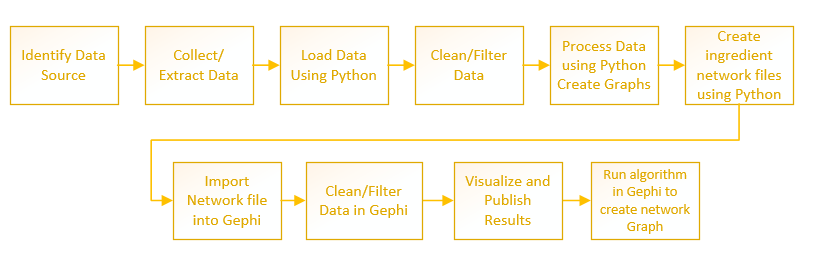
\includegraphics[width=\columnwidth]{images/methodology.PNG}
  \caption{Flowchart of the Methodology to Analyze Ingredients }\label{f:methodology}
\end{figure}


\subsection{Data Gathering}
The first step was to source the data. We were interested in the dataset which provides recipe information along with the ingredient used in the recipe. Since we wanted to analyze distribution across cuisines, data should also contain cuisine tagging. We evaluated 2 ways of gathering the data, generate the data ourselves or use publicly available data.  

The dataset can be generated by pulling recipe data from various online applications or pick from publicly available datasets. There are lot of applications online like allrecipes, Food, Yummly etc which hosts thousands of recipes and not to forget about recipe site available in every country, if we consider all these sources then it can easily contribute to huge dataset. Yannick Kimmel \cite{www-nyc} demonstrated in his recipe analysis project how recipe data can be source directly from the application. He did analysis of top 20 recipes from allrecipes website which is the largest web application hosting the recipes. He used Selenium package in Python to scarp allrecipes which can handle AJAX used in the application. Each recipe in allrecipe can be identified using unique identifier and follows generic format as allrecipes.com/recipe/[Unique ID number]. This generic URL is used by passing different unique id number to retrieve the recipe page and then find-element method is used to read various attributes like title, rating, reviews, calories per serving, prep time, cook time, total time and ingredients. We can follow the same approach to generate the dataset from different recipe sites for our analysis but we finalized publicly available dataset at Kaggle application satisfying need for this project to save the time.


\subsection{Dataset}
The dataset for this study is sourced from Kaggle application \cite{www-kaggle}. This dataset is publicly available and featured in \emph{What's Cooking?} competition. This dataset is provided to Kaggle by Yummly which is the application which hosts recipes online. This dataset is in JSON format and of 12MB size. This dataset contains recipe id, cuisine and list of ingredients as described in Figure \ref{c:data-structure}.
\begin{figure}[htb]
\begin{verbatim}
{
 "id": 24717,
 "cuisine": "indian",
 "ingredients": [
     "tumeric",
     "vegetable stock",
     "tomatoes",
     "garam masala",
     "naan",
     "red lentils",
     "red chili peppers",
     "onions",
     "spinach",
     "sweet potatoes"
 ]
 },
\end{verbatim}
\caption{Ingredient Data Structure}\label{c:data-structure}
\end{figure}
This dataset contains total 39774 recipes across various cuisines. We used two different methods to load this data. Cuisine and ingredient analysis is done by loading data into \emph{pandas dataframe} and to analyze ingredient relationship data has been loaded into \emph{json} object. Figure \ref{c:data-loading} shows the code for data loading used in this project.
\begin{figure}[htb]
\begin{verbatim}
#read the ingredient data using pandas
dfTrain = pd.read_json('./data/train.json')


#load data using json
dataFilePath="./data/train.json"
with open(dataFilePath) as data_file:    
    data = json.load(data_file)
\end{verbatim}
\caption{Data Loading}\label{c:data-loading}
\end{figure}

Ingredient extraction from the data structure and processing was challenging as ingredients are listed comma separated for each recipe. Also, ingredient list can vary by recipe and there is no proper structure. We observed shortcoming of dataset as
\begin{itemize}
\item \emph{Ingredient Duplication} - ingredient appears in the ingredient list in  various forms but it's the same ingredient which gives duplicate data. For example, salt appears as salt, kosher salt, Morton Salt, sea salt, table salt, Himalayan salt, fine sea salt, low sodium salt, fine salt. This is the same ingredient but come across in recipe as a different ingredient and getting counted as a separate ingredient in the analysis
\item \emph{Ingredient Name along with measure} - ingredients are listed along with measures like (10 oz.) frozen chopped spinach, (10 oz.) frozen chopped spinach, thawed and squeezed dry, (14.5 oz.) diced tomatoes and getting counted as a separate ingredient
\item \emph{Branded Ingredients} - ingredients are listed along with the brand name like KRAFT Reduced Fat Shredded Mozzarella Cheese, Johnsonville Smoked Sausage, Johnsonville Mild Italian Sausage Links etc and also constitutes to the ingredient list
\item \emph{Country Name with Ingredients} - ingredients are listed along with the country name like japanese cucumber, korean chile paste, Japanese soy sauce etc and also constitutes to the ingredient list
\item \emph{Ingredient name too long} - some ingredient name are too long to be an ingredient like \emph{wish-bone light asian sesame ginger vinaigrette dressing}
\item \emph{Ingredient with application} - ingredient names like chopped onion, diced tomatoes, chopped cilantro, grass-fed beef, grass-fed butter, cut up chicken
\end{itemize}

This variation makes difficult to get the proper ingredient list for the analysis. Extensive work is needed to clean and correct the noisy data so that proper analysis can be carried out. This correction process is not carried out as part of this project.

Certain ingredients like salt or water etc should be avoided from the analysis as those are not the ingredient we are looking for the analysis. We tried to clean such elements during ingredient relationship analysis but we had little success as those ingredients are present in the dataset in various forms.  

\subsection{Analysis and Findings}

\subsubsection{Recipe Distribution By Cuisine}
We first analyze entire dataset to understand the total number of recipes and their distribution across various cuisines. We use Pythons Panda library to get the total recipe count as 39774 and plot the distribution. Figure \ref{f:Number_of_recipes_by_cuisine} shows number of recipes per cuisine. Our observations from this analysis are
\begin{itemize}
\item Dataset is heavily dominated by Italian cuisine followed by Mexican cuisine which shows popularity of those cuisines
\item Very fewer recipes from Russian and Brazilian cuisines which shows very less contribution from those areas
\item No recipes from some regions like Germany, Canada which might be due to the recipes are not uploaded by users from that regions 
\item This also highlights another shortcoming of the dataset that it doesn't have equal representation of all cuisines which might give us biased analysis 
\end{itemize}
 
\begin{figure}[!ht]
  \centering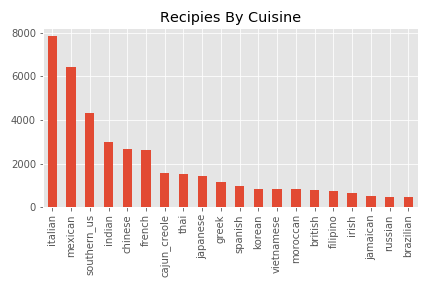
\includegraphics[width=\columnwidth]{images/Number_of_recipes_by_cuisine.png}
  \caption{Recipe Distribution By Cuisine }\label{f:Number_of_recipes_by_cuisine}
\end{figure}

Table\ref{t:recipecount} describes recipe count for every cuisine.
\begin{table}[htb]
\centering
\caption{Recipe Count By Cuisine}
\label{t:recipecount}
\begin{tabular}{ll}
Cuisine & Recipe Count \\
\hline
brazilian & 467 \\
british         &        804 \\
cajun creole    &       1546 \\
chinese         &       2673\\
filipino        &        755\\
french          &       2646\\
greek           &       1175\\
indian          &       3003\\
irish           &        667\\
italian         &       7838\\
jamaican        &        526\\
japanese        &       1423\\
korean          &        830\\
mexican         &       6438\\
moroccan        &        821\\
russian         &        489\\
southern us     &       4320\\
spanish         &        989\\
thai            &       1539\\
vietnamese      &        825\\

\end{tabular}
\end{table}

\subsubsection{Most Used Ingredients All Cuisines}
The second analysis is carried out to understand top 20 ingredients getting used across cuisine or globally. As per our study most used distinct ingredients across cuisines in order are
\begin{itemize}
\item Salt
\item Olive Oil
\item Onions
\item Water
\item Garlic
\item Sugar
\item Butter
\item Black Paper
\item All-purpose flour
\item Vegitable Oil
\item Eggs
\item Soy Sauce
\item Green Onions
\item Tomatoes
\item Carrots
\end{itemize}

Ingredient \emph{Salt} is obvious topper followed by \emph{Oil} and \emph{Onions}. This also proves our craving for salty and fatty food. Top 20 ingredient also contain duplicate ingredient like garlic and garlic clove, salt and kosher salt, eggs and large eggs which shows shortcoming of the dataset. Also ingredient like salt, oil and water could be avoided to get analysis of real ingredients as these are commonly use ingredient and doesn't contribute much to the study. Figure \ref{f:Ingredient_Distribution} shows top 20 ingredient across cuisines. 
\begin{figure}[!ht]
  \centering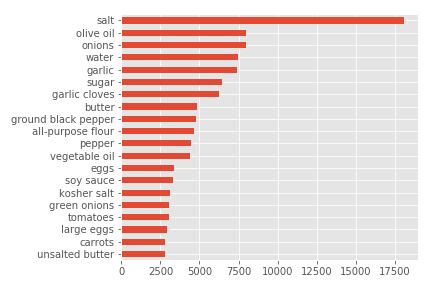
\includegraphics[width=\columnwidth]{images/Ingredient_Distribution.png}
  \caption{Top 20 Ingredients }\label{f:Ingredient_Distribution}
\end{figure}

\subsubsection{Ingredients Distribution By Cuisines}
The third analysis is carried out to understand key ingredient for each cuisine. These key ingredients define those cuisines and provide unique test characterized by that cuisine. We limited ingredient list to top 10 to get the key ingredients for each cuisine. Study shows key ingredient for our top 5 cuisines as follows
\begin{itemize}
\item \emph{Italian} - Olive oil, garlic, cheese, black pepper, onion and butter
\item \emph{Mexican} - onion, cumin, garlic, chili powder, jalapeno chilies, sour cream, tortillas and avocado
\item \emph{Southern US} - butter, all-purpose flour, sugar, eggs, baking powder, milk and butter milk
\item \emph{Indian} - onion, garam masala, turmeric, garlic, cumin and oil
\item \emph{Chinese} - soy sauce, sesame oil, corn starch, sugar, garlic, green onions and scallions
\end{itemize}

Similarly we show key ingredient of all other cuisines present in the dataset and we observe that it is very close representation of all cuisines. Figure \ref{f:italian_10_most_used_ingredients}, \ref{f:brazilian_10_most_used_ingredients}, \ref{f:british_10_most_used_ingredients}, \ref{f:cajun_creole_10_most_used_ingredients}, \ref{f:chinese_10_most_used_ingredients}, \ref{f:filipino_10_most_used_ingredients}, \ref{f:french_10_most_used_ingredients}, \ref{f:greek_10_most_used_ingredients}, \ref{f:indian_10_most_used_ingredients}, \ref{f:irish_10_most_used_ingredients}, \ref{f:jamaican_10_most_used_ingredients}, \ref{f:japanese_10_most_used_ingredients}, \ref{f:korean_10_most_used_ingredients}, \ref{f:mexican_10_most_used_ingredients}, \ref{f:moroccan_10_most_used_ingredients}, \ref{f:russian_10_most_used_ingredients}, \ref{f:southern_us_10_most_used_ingredients}, \ref{f:spanish_10_most_used_ingredients}, \ref{f:thai_10_most_used_ingredients}, \ref{f:vietnamese_10_most_used_ingredients}  shows top 10 key ingredient used in the corresponding cuisines. 
\begin{figure}[!ht]
  \centering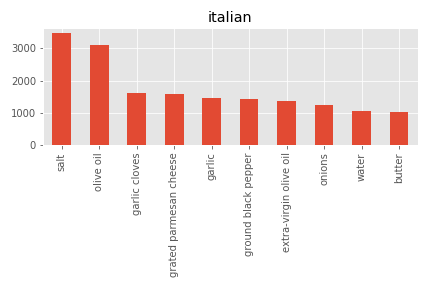
\includegraphics[width=\columnwidth]{images/italian_10_most_used_ingredients.png}
  \caption{Top 10 Ingredients }\label{f:italian_10_most_used_ingredients}
\end{figure}

\begin{figure}[!ht]
  \centering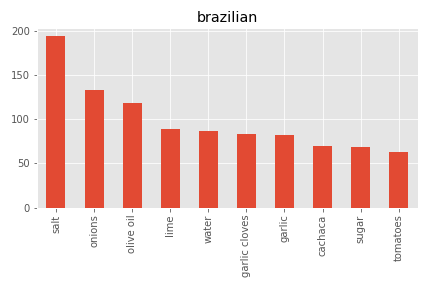
\includegraphics[width=\columnwidth]{images/brazilian_10_most_used_ingredients.png}
  \caption{Top 10 Ingredients }\label{f:brazilian_10_most_used_ingredients}
\end{figure}

\begin{figure}[!ht]
  \centering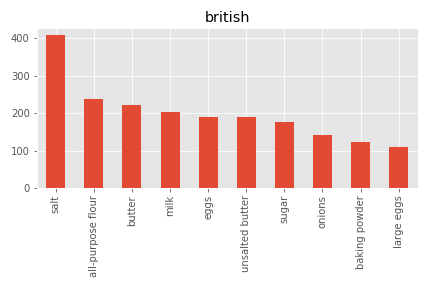
\includegraphics[width=\columnwidth]{images/british_10_most_used_ingredients.png}
  \caption{Top 10 Ingredients }\label{f:british_10_most_used_ingredients}
\end{figure}

\begin{figure}[!ht]
  \centering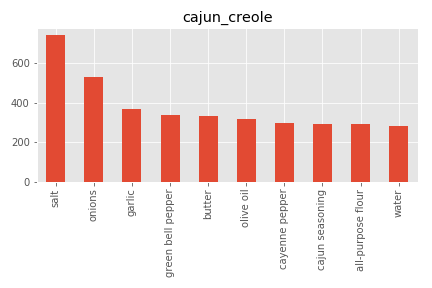
\includegraphics[width=\columnwidth]{images/cajun_creole_10_most_used_ingredients.png}
  \caption{Top 10 Ingredients }\label{f:cajun_creole_10_most_used_ingredients}
\end{figure}

\begin{figure}[!ht]
  \centering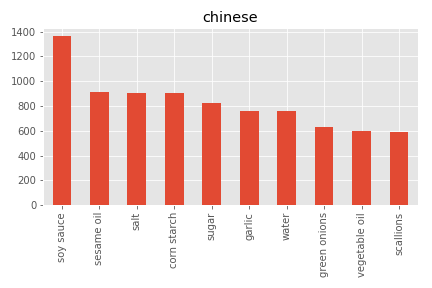
\includegraphics[width=\columnwidth]{images/chinese_10_most_used_ingredients.png}
  \caption{Top 10 Ingredients }\label{f:chinese_10_most_used_ingredients}
\end{figure}

\begin{figure}[!ht]
  \centering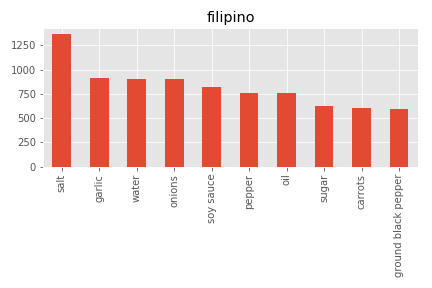
\includegraphics[width=\columnwidth]{images/filipino_10_most_used_ingredients.png}
  \caption{Top 10 Ingredients }\label{f:filipino_10_most_used_ingredients}
\end{figure}

\begin{figure}[!ht]
  \centering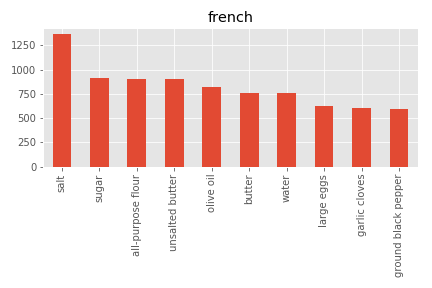
\includegraphics[width=\columnwidth]{images/french_10_most_used_ingredients.png}
  \caption{Top 10 Ingredients }\label{f:french_10_most_used_ingredients}
\end{figure}

\begin{figure}[!ht]
  \centering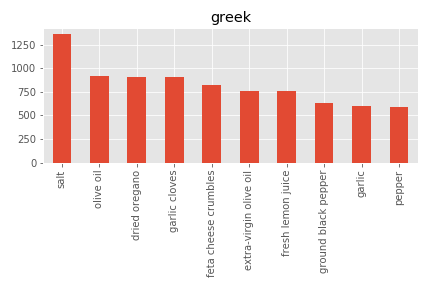
\includegraphics[width=\columnwidth]{images/greek_10_most_used_ingredients.png}
  \caption{Top 10 Ingredients }\label{f:greek_10_most_used_ingredients}
\end{figure}

\begin{figure}[!ht]
  \centering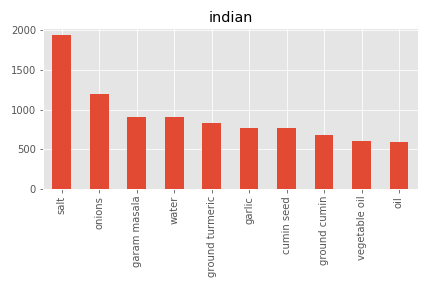
\includegraphics[width=\columnwidth]{images/indian_10_most_used_ingredients.png}
  \caption{Top 10 Ingredients }\label{f:indian_10_most_used_ingredients}
\end{figure}

\begin{figure}[!ht]
  \centering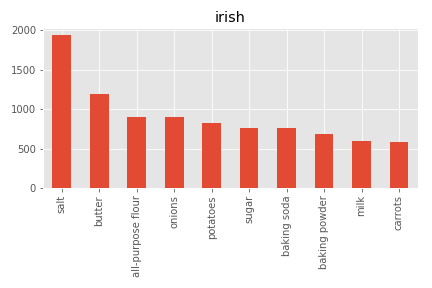
\includegraphics[width=\columnwidth]{images/irish_10_most_used_ingredients.png}
  \caption{Top 10 Ingredients }\label{f:irish_10_most_used_ingredients}
\end{figure}

\begin{figure}[!ht]
  \centering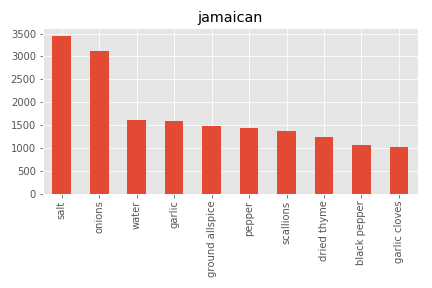
\includegraphics[width=\columnwidth]{images/jamaican_10_most_used_ingredients.png}
  \caption{Top 10 Ingredients }\label{f:jamaican_10_most_used_ingredients}
\end{figure}

\begin{figure}[!ht]
  \centering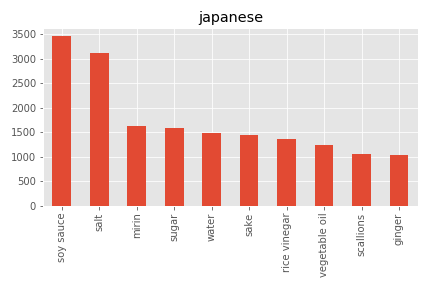
\includegraphics[width=\columnwidth]{images/japanese_10_most_used_ingredients.png}
  \caption{Top 10 Ingredients }\label{f:japanese_10_most_used_ingredients}
\end{figure}

\begin{figure}[!ht]
  \centering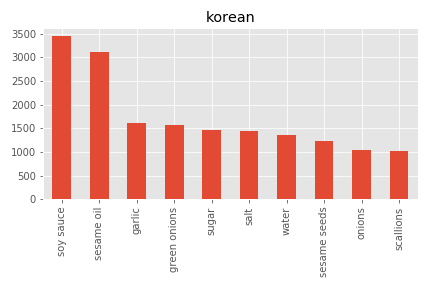
\includegraphics[width=\columnwidth]{images/korean_10_most_used_ingredients.png}
  \caption{Top 10 Ingredients }\label{f:korean_10_most_used_ingredients}
\end{figure}

\begin{figure}[!ht]
  \centering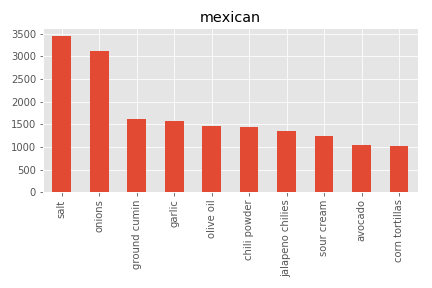
\includegraphics[width=\columnwidth]{images/mexican_10_most_used_ingredients.png}
  \caption{Top 10 Ingredients }\label{f:mexican_10_most_used_ingredients}
\end{figure}

\begin{figure}[!ht]
  \centering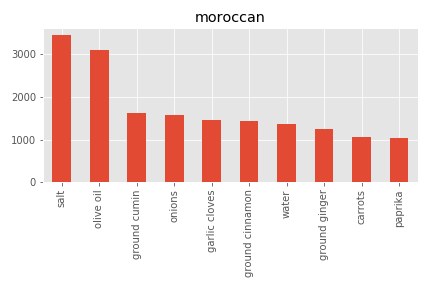
\includegraphics[width=\columnwidth]{images/moroccan_10_most_used_ingredients.png}
  \caption{Top 10 Ingredients }\label{f:moroccan_10_most_used_ingredients}
\end{figure}

\begin{figure}[!ht]
  \centering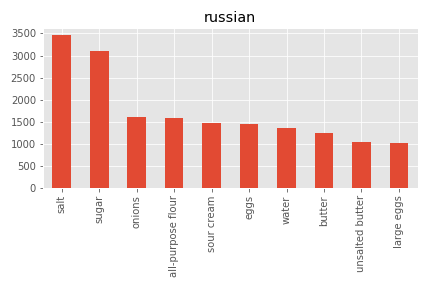
\includegraphics[width=\columnwidth]{images/russian_10_most_used_ingredients.png}
  \caption{Top 10 Ingredients }\label{f:russian_10_most_used_ingredients}
\end{figure}

\begin{figure}[!ht]
  \centering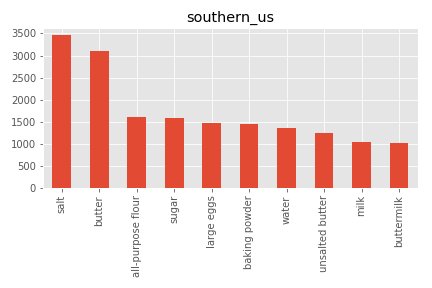
\includegraphics[width=\columnwidth]{images/southern_us_10_most_used_ingredients.png}
  \caption{Top 10 Ingredients }\label{f:southern_us_10_most_used_ingredients}
\end{figure}

\begin{figure}[!ht]
  \centering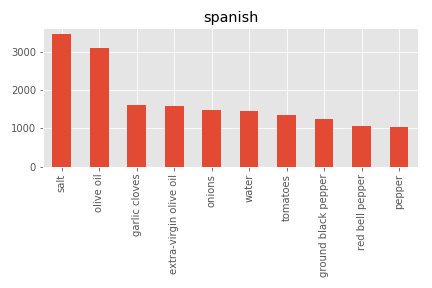
\includegraphics[width=\columnwidth]{images/spanish_10_most_used_ingredients.png}
  \caption{Top 10 Ingredients }\label{f:spanish_10_most_used_ingredients}
\end{figure}

\begin{figure}[!ht]
  \centering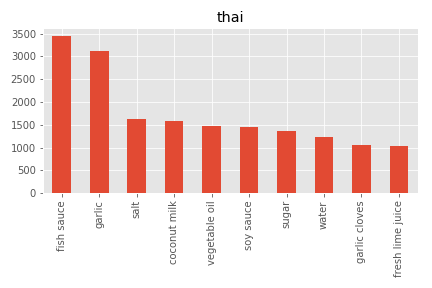
\includegraphics[width=\columnwidth]{images/thai_10_most_used_ingredients.png}
  \caption{Top 10 Ingredients }\label{f:thai_10_most_used_ingredients}
\end{figure}

\begin{figure}[!ht]
  \centering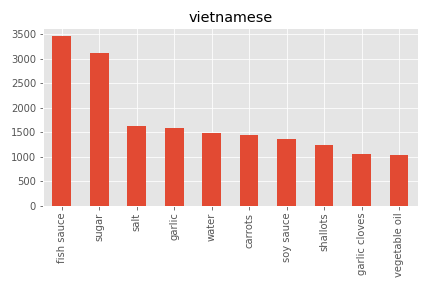
\includegraphics[width=\columnwidth]{images/vietnamese_10_most_used_ingredients.png}
  \caption{Top 10 Ingredients }\label{f:vietnamese_10_most_used_ingredients}
\end{figure}


\subsubsection{Ingredients Relationship}
Forth analysis is carried out to understand the relationship between the ingredient to find out ingredient clusters. This analysis helps us understand the ingredient combinations which can be used together to provide great dish every time. This model can be used to predict ingredients for certain recipe based on the cluster. We used Gephi tool to analyze and produce the graph for this analysis. Gephi accepts network structure in terms of Node and Edge relationship. We created this network using python by relating all ingredients present in the recipe with each other. Ingredients become the node and source and target nodes become the edges. These network files generated in excel spreadsheet and converted to CSV format and imported into the Gephi tool. Import created 5405 Nodes and 290828 edges for processing and analysis. Force Atlas 2 layout present in Gephi has been applied to the network which brings nodes with higher weights and shared connections closer to each other. We also used Gephi Data Laboratory to clean up duplicate or unwanted nodes. Filtering based on Degree Range and Edge Weight has been applied to data to reduce node and edges to get the graph which can be used for analysis and avoid crashing Gephi due to large data. Modularity statistic uncovered 5 ingredient clusters which can be identified by different colors in the graph. This cluster can approximately related to the cuisines present in our dataset and confirms our earlier analysis of ingredient by cuisine.
\begin{itemize}
\item Orange - Mexican
\item Brown  - Indian
\item Blue   - Chinese
\item Green  - Italian
\item Gray   - Southern US
\end{itemize}

This analysis also provides us with the complimentary ingredient network which can be used together to construct tasty dish. We can see that there are two type of combination one is savoury and another is sweet. The complimentary ingredients as per our study are
\begin{itemize}
\item Sugar, butter, all-purpose flour, large eggs, heavy cream, baking powder, cinnamon, flour, lemon, vanilla
\item Olive oil, garlic, black paper, onion, cheese, basil, parsley, oregano, white wine, shallots, lemon juice, bell paper
\item Onion, garlic, pepper, tomato, bay leaves, paprika, potatoes, chicken, shrimp, celery, green paper, garlic powder, dried thyme
\item Tomato, ground cumin, chicken, cilantro, jalapeno chilies, ground beef, sour cream, chili powder, avocado, corn tortillas, black beans, salsa, lime, green chilies, oil, turmeric, garam masala, coconut milk
\item Oil, green onions, scallions, carrots, garlic, ginger, fish sauce, soy sauce, rice vinegar, sesame oil, corn starch, brown sugar, honey
\end{itemize}

Graph also shows overlap between following ingredients which confirms that those are  the commonly together used ingredients in the recipes. We observe those combination in Indian and Italian cuisine. 
\begin{itemize}
\item Onion, garlic
\item Olive oil, black paper
\end{itemize}

Figure \ref{f:ingredient_modularity} shows ingredient cluster of more than 1000 nodes. This graph is nice to look at but difficult to read due to lot many nodes and edges in the graph. 
\begin{figure}[!ht]
  \centering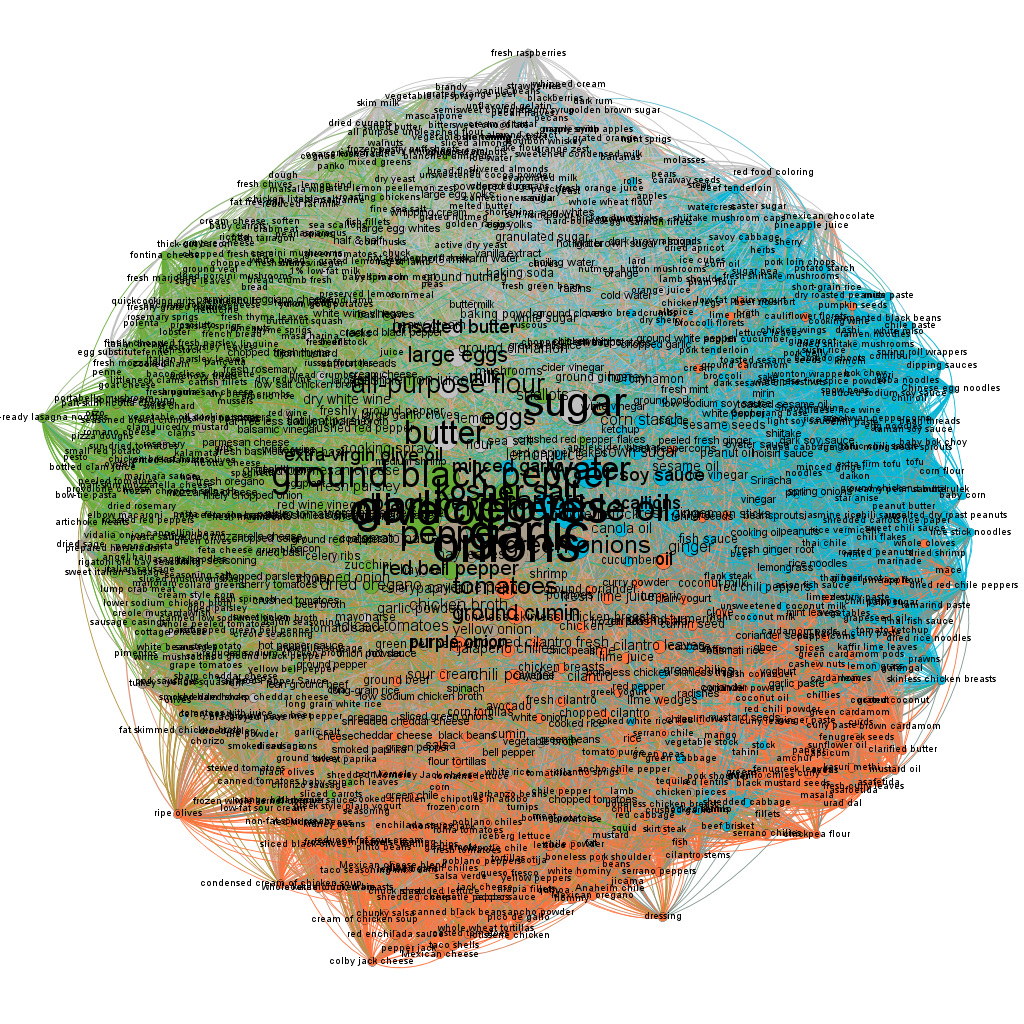
\includegraphics[width=\columnwidth]{images/ingredient_modularity.png}
  \caption{Ingredient Cluster }\label{f:ingredient_modularity}
\end{figure}

Figure \ref{f:ingredient_modularity100} shows ingredient cluster of around 100 nodes. We generated this graph by reducing nodes and edges to make it more readable. This graph provides us with our top 5 cuisine clusters.  
\begin{figure}[!ht]
  \centering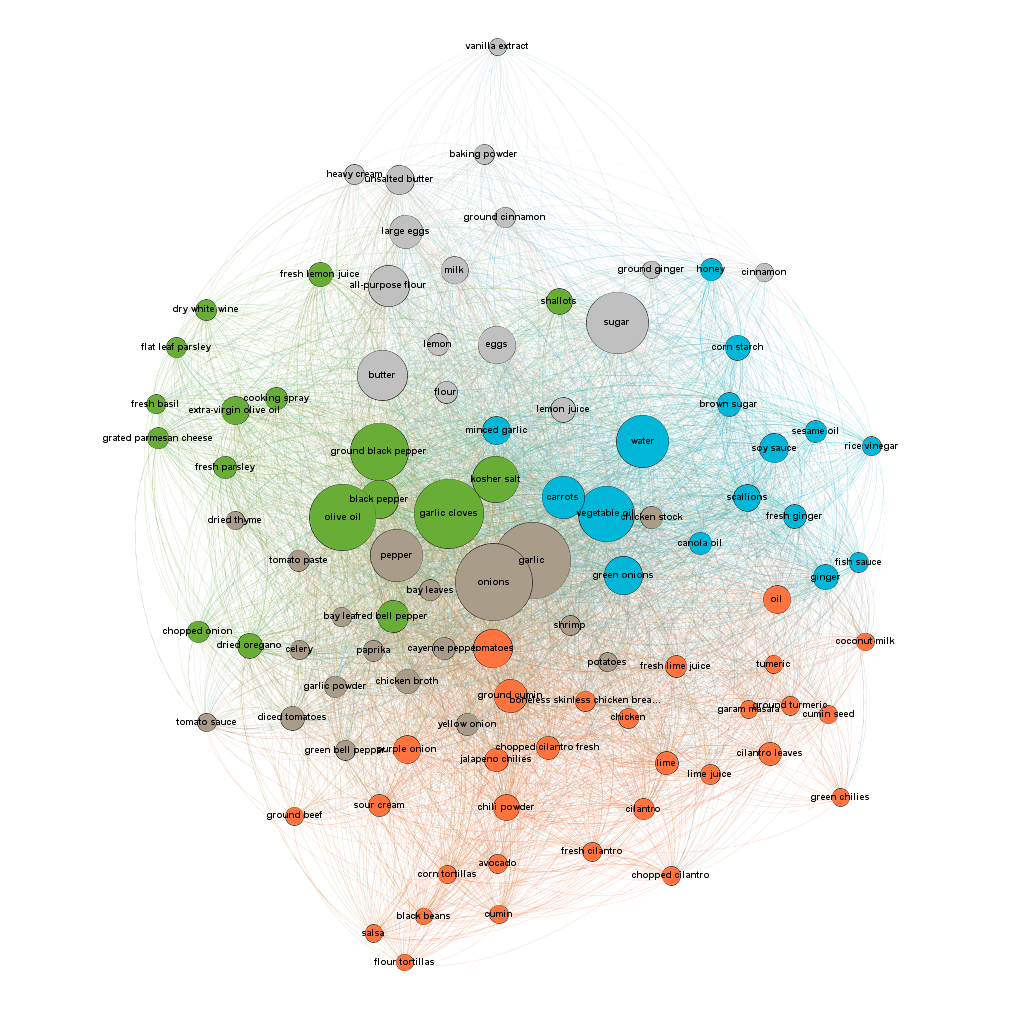
\includegraphics[width=\columnwidth]{images/ingredient_modularity100.png}
  \caption{ingredient Cluster 100 Nodes }\label{f:ingredient_modularity100}
\end{figure}

\subsection{Shortcomings}
Improper documentation of ingredient names in the dataset reduces the correctness of this analysis. In absence of proper ingredient name and duplication of ingredient name prevents getting exact ingredient weight into the analysis. A dataset with uniform ingredient name can help this analysis to achieve its best. If we don't find proper ingredient name then this analysis needs to include extensive data cleaning process which can be considered an improvement to this project.

Network file creation algorithm can be enhanced further by considering the number of recipes for the ingredient to provide additional weight to the relationship which can provide the stronger bond between the ingredients. 

\subsection{Limitations}
This dataset can be analyzed to find out ingredient overlap between various cuisine and can provide insight into the influence of one cuisine on another which is not covered as part of this study. Usually, geographically neighboring cuisines are influenced by each other as they share common ingredients. 

\section{Conclusion}
This project shows most used ingredient, ingredient distribution by cuisine and predictive ingredient relationship model as per the goal of the project. We also show various opportunities present with ingredient data analysis and role of big data analytics. We prove human craving for salty and fatty food as salt and oil are most used ingredient across cuisines as per the analysis. We understand now based on our analysis key ingredient of any cuisine. Ingredient cluster shows why those ingredients are the base of certain cuisine and recipe of those ingredients always turn out delicious. We also crave for the good data so that we can provide more accurate analysis of the ingredients. Ingredient analysis has potential not only to help restaurant and food industry but it can help with our social responsibility of sustainability and understanding different cuisines and culture. As food industries interest grows in big data analytics, we will continue to see more evaluations of the ingredients.  

\begin{acks}
  The author would like to thank Dr. Gregor von Laszewski for his support and suggestions in this project. The author would also like to acknowledge Kaggle application for hosting ingredient dataset which is used in this project and various application users contributing in data analysis. We also acknowledge various online resources which helped understand Python and Gephi.  
\end{acks}

\bibliographystyle{ACM-Reference-Format}
\bibliography{report} 

\appendix



\end{document}
